% Created by tikzDevice version 0.12.6 on 2025-04-17 10:36:45
% !TEX encoding = UTF-8 Unicode
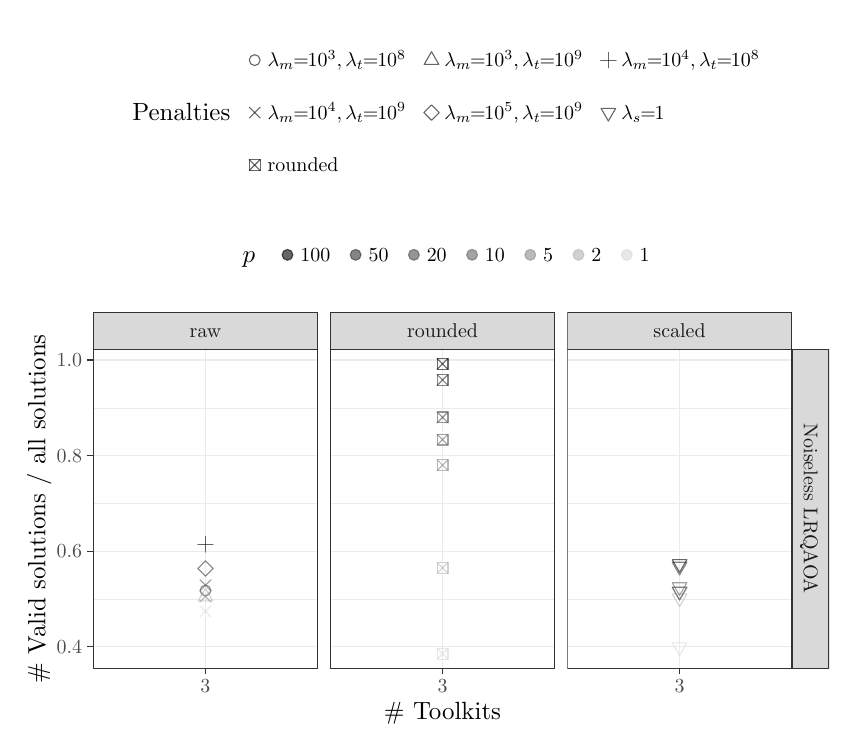
\begin{tikzpicture}[x=1pt,y=1pt]
\definecolor{fillColor}{RGB}{255,255,255}
\path[use as bounding box,fill=fillColor,fill opacity=0.00] (0,0) rectangle (289.58,251.81);
\begin{scope}
\path[clip] (  0.00,  0.00) rectangle (289.58,251.81);
\definecolor{drawColor}{RGB}{255,255,255}
\definecolor{fillColor}{RGB}{255,255,255}

\path[draw=drawColor,line width= 0.5pt,line join=round,line cap=round,fill=fillColor] (  0.00,  0.00) rectangle (289.58,251.81);
\end{scope}
\begin{scope}
\path[clip] ( 23.68, 20.35) rectangle (104.83,135.55);
\definecolor{fillColor}{RGB}{255,255,255}

\path[fill=fillColor] ( 23.68, 20.35) rectangle (104.83,135.55);
\definecolor{drawColor}{gray}{0.92}

\path[draw=drawColor,line width= 0.2pt,line join=round] ( 23.68, 45.36) --
	(104.83, 45.36);

\path[draw=drawColor,line width= 0.2pt,line join=round] ( 23.68, 79.88) --
	(104.83, 79.88);

\path[draw=drawColor,line width= 0.2pt,line join=round] ( 23.68,114.40) --
	(104.83,114.40);

\path[draw=drawColor,line width= 0.5pt,line join=round] ( 23.68, 28.10) --
	(104.83, 28.10);

\path[draw=drawColor,line width= 0.5pt,line join=round] ( 23.68, 62.62) --
	(104.83, 62.62);

\path[draw=drawColor,line width= 0.5pt,line join=round] ( 23.68, 97.14) --
	(104.83, 97.14);

\path[draw=drawColor,line width= 0.5pt,line join=round] ( 23.68,131.66) --
	(104.83,131.66);

\path[draw=drawColor,line width= 0.5pt,line join=round] ( 64.25, 20.35) --
	( 64.25,135.55);
\definecolor{drawColor}{RGB}{102,102,102}

\path[draw=drawColor,draw opacity=0.60,line width= 0.4pt,line join=round,line cap=round] ( 62.29, 48.37) -- ( 66.21, 52.29);

\path[draw=drawColor,draw opacity=0.60,line width= 0.4pt,line join=round,line cap=round] ( 62.29, 52.29) -- ( 66.21, 48.37);
\definecolor{drawColor}{RGB}{77,77,77}

\path[draw=drawColor,draw opacity=0.60,line width= 0.4pt,line join=round,line cap=round] ( 64.25, 48.43) circle (  1.96);
\definecolor{drawColor}{RGB}{217,217,217}

\path[draw=drawColor,draw opacity=0.60,line width= 0.4pt,line join=round,line cap=round] ( 62.29, 38.91) -- ( 66.21, 42.84);

\path[draw=drawColor,draw opacity=0.60,line width= 0.4pt,line join=round,line cap=round] ( 62.29, 42.84) -- ( 66.21, 38.91);
\definecolor{drawColor}{RGB}{179,179,179}

\path[draw=drawColor,draw opacity=0.60,line width= 0.4pt,line join=round,line cap=round] ( 64.25, 49.23) --
	( 66.89, 44.66) --
	( 61.61, 44.66) --
	cycle;
\definecolor{drawColor}{RGB}{140,140,140}

\path[draw=drawColor,draw opacity=0.60,line width= 0.4pt,line join=round,line cap=round] ( 62.29, 44.31) -- ( 66.21, 48.23);

\path[draw=drawColor,draw opacity=0.60,line width= 0.4pt,line join=round,line cap=round] ( 62.29, 48.23) -- ( 66.21, 44.31);
\definecolor{drawColor}{RGB}{51,51,51}

\path[draw=drawColor,draw opacity=0.60,line width= 0.4pt,line join=round,line cap=round] ( 61.48, 56.38) --
	( 64.25, 59.16) --
	( 67.03, 56.38) --
	( 64.25, 53.61) --
	cycle;
\definecolor{drawColor}{RGB}{0,0,0}

\path[draw=drawColor,draw opacity=0.60,line width= 0.4pt,line join=round,line cap=round] ( 61.48, 65.10) -- ( 67.03, 65.10);

\path[draw=drawColor,draw opacity=0.60,line width= 0.4pt,line join=round,line cap=round] ( 64.25, 62.32) -- ( 64.25, 67.87);
\definecolor{drawColor}{gray}{0.20}

\path[draw=drawColor,line width= 0.5pt,line join=round,line cap=round] ( 23.68, 20.35) rectangle (104.83,135.55);
\end{scope}
\begin{scope}
\path[clip] (109.33, 20.35) rectangle (190.48,135.55);
\definecolor{fillColor}{RGB}{255,255,255}

\path[fill=fillColor] (109.33, 20.35) rectangle (190.48,135.55);
\definecolor{drawColor}{gray}{0.92}

\path[draw=drawColor,line width= 0.2pt,line join=round] (109.33, 45.36) --
	(190.48, 45.36);

\path[draw=drawColor,line width= 0.2pt,line join=round] (109.33, 79.88) --
	(190.48, 79.88);

\path[draw=drawColor,line width= 0.2pt,line join=round] (109.33,114.40) --
	(190.48,114.40);

\path[draw=drawColor,line width= 0.5pt,line join=round] (109.33, 28.10) --
	(190.48, 28.10);

\path[draw=drawColor,line width= 0.5pt,line join=round] (109.33, 62.62) --
	(190.48, 62.62);

\path[draw=drawColor,line width= 0.5pt,line join=round] (109.33, 97.14) --
	(190.48, 97.14);

\path[draw=drawColor,line width= 0.5pt,line join=round] (109.33,131.66) --
	(190.48,131.66);

\path[draw=drawColor,line width= 0.5pt,line join=round] (149.90, 20.35) --
	(149.90,135.55);
\definecolor{drawColor}{RGB}{0,0,0}

\path[draw=drawColor,draw opacity=0.60,line width= 0.4pt,line join=round,line cap=round] (147.94,128.35) rectangle (151.87,132.27);

\path[draw=drawColor,draw opacity=0.60,line width= 0.4pt,line join=round,line cap=round] (147.94,128.35) -- (151.87,132.27);

\path[draw=drawColor,draw opacity=0.60,line width= 0.4pt,line join=round,line cap=round] (147.94,132.27) -- (151.87,128.35);
\definecolor{drawColor}{RGB}{140,140,140}

\path[draw=drawColor,draw opacity=0.60,line width= 0.4pt,line join=round,line cap=round] (147.94, 91.74) rectangle (151.87, 95.66);

\path[draw=drawColor,draw opacity=0.60,line width= 0.4pt,line join=round,line cap=round] (147.94, 91.74) -- (151.87, 95.66);

\path[draw=drawColor,draw opacity=0.60,line width= 0.4pt,line join=round,line cap=round] (147.94, 95.66) -- (151.87, 91.74);
\definecolor{drawColor}{RGB}{102,102,102}

\path[draw=drawColor,draw opacity=0.60,line width= 0.4pt,line join=round,line cap=round] (147.94,100.99) rectangle (151.87,104.91);

\path[draw=drawColor,draw opacity=0.60,line width= 0.4pt,line join=round,line cap=round] (147.94,100.99) -- (151.87,104.91);

\path[draw=drawColor,draw opacity=0.60,line width= 0.4pt,line join=round,line cap=round] (147.94,104.91) -- (151.87,100.99);
\definecolor{drawColor}{RGB}{77,77,77}

\path[draw=drawColor,draw opacity=0.60,line width= 0.4pt,line join=round,line cap=round] (147.94,108.99) rectangle (151.87,112.92);

\path[draw=drawColor,draw opacity=0.60,line width= 0.4pt,line join=round,line cap=round] (147.94,108.99) -- (151.87,112.92);

\path[draw=drawColor,draw opacity=0.60,line width= 0.4pt,line join=round,line cap=round] (147.94,112.92) -- (151.87,108.99);
\definecolor{drawColor}{RGB}{179,179,179}

\path[draw=drawColor,draw opacity=0.60,line width= 0.4pt,line join=round,line cap=round] (147.94, 54.65) rectangle (151.87, 58.57);

\path[draw=drawColor,draw opacity=0.60,line width= 0.4pt,line join=round,line cap=round] (147.94, 54.65) -- (151.87, 58.57);

\path[draw=drawColor,draw opacity=0.60,line width= 0.4pt,line join=round,line cap=round] (147.94, 58.57) -- (151.87, 54.65);
\definecolor{drawColor}{RGB}{217,217,217}

\path[draw=drawColor,draw opacity=0.60,line width= 0.4pt,line join=round,line cap=round] (147.94, 23.63) rectangle (151.87, 27.55);

\path[draw=drawColor,draw opacity=0.60,line width= 0.4pt,line join=round,line cap=round] (147.94, 23.63) -- (151.87, 27.55);

\path[draw=drawColor,draw opacity=0.60,line width= 0.4pt,line join=round,line cap=round] (147.94, 27.55) -- (151.87, 23.63);
\definecolor{drawColor}{RGB}{51,51,51}

\path[draw=drawColor,draw opacity=0.60,line width= 0.4pt,line join=round,line cap=round] (147.94,122.55) rectangle (151.87,126.47);

\path[draw=drawColor,draw opacity=0.60,line width= 0.4pt,line join=round,line cap=round] (147.94,122.55) -- (151.87,126.47);

\path[draw=drawColor,draw opacity=0.60,line width= 0.4pt,line join=round,line cap=round] (147.94,126.47) -- (151.87,122.55);
\definecolor{drawColor}{gray}{0.20}

\path[draw=drawColor,line width= 0.5pt,line join=round,line cap=round] (109.33, 20.35) rectangle (190.48,135.55);
\end{scope}
\begin{scope}
\path[clip] (194.98, 20.35) rectangle (276.13,135.55);
\definecolor{fillColor}{RGB}{255,255,255}

\path[fill=fillColor] (194.98, 20.35) rectangle (276.13,135.55);
\definecolor{drawColor}{gray}{0.92}

\path[draw=drawColor,line width= 0.2pt,line join=round] (194.98, 45.36) --
	(276.13, 45.36);

\path[draw=drawColor,line width= 0.2pt,line join=round] (194.98, 79.88) --
	(276.13, 79.88);

\path[draw=drawColor,line width= 0.2pt,line join=round] (194.98,114.40) --
	(276.13,114.40);

\path[draw=drawColor,line width= 0.5pt,line join=round] (194.98, 28.10) --
	(276.13, 28.10);

\path[draw=drawColor,line width= 0.5pt,line join=round] (194.98, 62.62) --
	(276.13, 62.62);

\path[draw=drawColor,line width= 0.5pt,line join=round] (194.98, 97.14) --
	(276.13, 97.14);

\path[draw=drawColor,line width= 0.5pt,line join=round] (194.98,131.66) --
	(276.13,131.66);

\path[draw=drawColor,line width= 0.5pt,line join=round] (235.56, 20.35) --
	(235.56,135.55);
\definecolor{drawColor}{RGB}{217,217,217}

\path[draw=drawColor,draw opacity=0.60,line width= 0.4pt,line join=round,line cap=round] (235.56, 24.94) --
	(238.20, 29.52) --
	(232.91, 29.52) --
	cycle;
\definecolor{drawColor}{RGB}{179,179,179}

\path[draw=drawColor,draw opacity=0.60,line width= 0.4pt,line join=round,line cap=round] (235.56, 42.61) --
	(238.20, 47.19) --
	(232.91, 47.19) --
	cycle;
\definecolor{drawColor}{RGB}{140,140,140}

\path[draw=drawColor,draw opacity=0.60,line width= 0.4pt,line join=round,line cap=round] (235.56, 45.12) --
	(238.20, 49.70) --
	(232.91, 49.70) --
	cycle;
\definecolor{drawColor}{RGB}{77,77,77}

\path[draw=drawColor,draw opacity=0.60,line width= 0.4pt,line join=round,line cap=round] (235.56, 44.96) --
	(238.20, 49.54) --
	(232.91, 49.54) --
	cycle;
\definecolor{drawColor}{RGB}{51,51,51}

\path[draw=drawColor,draw opacity=0.60,line width= 0.4pt,line join=round,line cap=round] (235.56, 54.05) --
	(238.20, 58.63) --
	(232.91, 58.63) --
	cycle;
\definecolor{drawColor}{RGB}{102,102,102}

\path[draw=drawColor,draw opacity=0.60,line width= 0.4pt,line join=round,line cap=round] (235.56, 46.66) --
	(238.20, 51.23) --
	(232.91, 51.23) --
	cycle;
\definecolor{drawColor}{RGB}{0,0,0}

\path[draw=drawColor,draw opacity=0.60,line width= 0.4pt,line join=round,line cap=round] (235.56, 54.99) --
	(238.20, 59.57) --
	(232.91, 59.57) --
	cycle;
\definecolor{drawColor}{gray}{0.20}

\path[draw=drawColor,line width= 0.5pt,line join=round,line cap=round] (194.98, 20.35) rectangle (276.13,135.55);
\end{scope}
\begin{scope}
\path[clip] ( 23.68,135.55) rectangle (104.83,148.99);
\definecolor{drawColor}{gray}{0.20}
\definecolor{fillColor}{gray}{0.85}

\path[draw=drawColor,line width= 0.5pt,line join=round,line cap=round,fill=fillColor] ( 23.68,135.55) rectangle (104.83,148.99);
\definecolor{drawColor}{gray}{0.10}

\node[text=drawColor,anchor=base,inner sep=0pt, outer sep=0pt, scale=  0.72] at ( 64.25,139.92) {raw};
\end{scope}
\begin{scope}
\path[clip] (109.33,135.55) rectangle (190.48,148.99);
\definecolor{drawColor}{gray}{0.20}
\definecolor{fillColor}{gray}{0.85}

\path[draw=drawColor,line width= 0.5pt,line join=round,line cap=round,fill=fillColor] (109.33,135.55) rectangle (190.48,148.99);
\definecolor{drawColor}{gray}{0.10}

\node[text=drawColor,anchor=base,inner sep=0pt, outer sep=0pt, scale=  0.72] at (149.90,139.92) {rounded};
\end{scope}
\begin{scope}
\path[clip] (194.98,135.55) rectangle (276.13,148.99);
\definecolor{drawColor}{gray}{0.20}
\definecolor{fillColor}{gray}{0.85}

\path[draw=drawColor,line width= 0.5pt,line join=round,line cap=round,fill=fillColor] (194.98,135.55) rectangle (276.13,148.99);
\definecolor{drawColor}{gray}{0.10}

\node[text=drawColor,anchor=base,inner sep=0pt, outer sep=0pt, scale=  0.72] at (235.56,139.92) {scaled};
\end{scope}
\begin{scope}
\path[clip] (276.13, 20.35) rectangle (289.58,135.55);
\definecolor{drawColor}{gray}{0.20}
\definecolor{fillColor}{gray}{0.85}

\path[draw=drawColor,line width= 0.5pt,line join=round,line cap=round,fill=fillColor] (276.13, 20.35) rectangle (289.58,135.55);
\definecolor{drawColor}{gray}{0.10}

\node[text=drawColor,rotate=-90.00,anchor=base,inner sep=0pt, outer sep=0pt, scale=  0.72] at (280.51, 77.95) {Noiseless LRQAOA};
\end{scope}
\begin{scope}
\path[clip] (  0.00,  0.00) rectangle (289.58,251.81);
\definecolor{drawColor}{gray}{0.20}

\path[draw=drawColor,line width= 0.5pt,line join=round] ( 64.25, 18.10) --
	( 64.25, 20.35);
\end{scope}
\begin{scope}
\path[clip] (  0.00,  0.00) rectangle (289.58,251.81);
\definecolor{drawColor}{gray}{0.30}

\node[text=drawColor,anchor=base,inner sep=0pt, outer sep=0pt, scale=  0.72] at ( 64.25, 11.62) {3};
\end{scope}
\begin{scope}
\path[clip] (  0.00,  0.00) rectangle (289.58,251.81);
\definecolor{drawColor}{gray}{0.20}

\path[draw=drawColor,line width= 0.5pt,line join=round] (149.90, 18.10) --
	(149.90, 20.35);
\end{scope}
\begin{scope}
\path[clip] (  0.00,  0.00) rectangle (289.58,251.81);
\definecolor{drawColor}{gray}{0.30}

\node[text=drawColor,anchor=base,inner sep=0pt, outer sep=0pt, scale=  0.72] at (149.90, 11.62) {3};
\end{scope}
\begin{scope}
\path[clip] (  0.00,  0.00) rectangle (289.58,251.81);
\definecolor{drawColor}{gray}{0.20}

\path[draw=drawColor,line width= 0.5pt,line join=round] (235.56, 18.10) --
	(235.56, 20.35);
\end{scope}
\begin{scope}
\path[clip] (  0.00,  0.00) rectangle (289.58,251.81);
\definecolor{drawColor}{gray}{0.30}

\node[text=drawColor,anchor=base,inner sep=0pt, outer sep=0pt, scale=  0.72] at (235.56, 11.62) {3};
\end{scope}
\begin{scope}
\path[clip] (  0.00,  0.00) rectangle (289.58,251.81);
\definecolor{drawColor}{gray}{0.30}

\node[text=drawColor,anchor=base east,inner sep=0pt, outer sep=0pt, scale=  0.72] at ( 19.63, 25.76) {0.4};

\node[text=drawColor,anchor=base east,inner sep=0pt, outer sep=0pt, scale=  0.72] at ( 19.63, 60.28) {0.6};

\node[text=drawColor,anchor=base east,inner sep=0pt, outer sep=0pt, scale=  0.72] at ( 19.63, 94.80) {0.8};

\node[text=drawColor,anchor=base east,inner sep=0pt, outer sep=0pt, scale=  0.72] at ( 19.63,129.31) {1.0};
\end{scope}
\begin{scope}
\path[clip] (  0.00,  0.00) rectangle (289.58,251.81);
\definecolor{drawColor}{gray}{0.20}

\path[draw=drawColor,line width= 0.5pt,line join=round] ( 21.43, 28.10) --
	( 23.68, 28.10);

\path[draw=drawColor,line width= 0.5pt,line join=round] ( 21.43, 62.62) --
	( 23.68, 62.62);

\path[draw=drawColor,line width= 0.5pt,line join=round] ( 21.43, 97.14) --
	( 23.68, 97.14);

\path[draw=drawColor,line width= 0.5pt,line join=round] ( 21.43,131.66) --
	( 23.68,131.66);
\end{scope}
\begin{scope}
\path[clip] (  0.00,  0.00) rectangle (289.58,251.81);
\definecolor{drawColor}{RGB}{0,0,0}

\node[text=drawColor,anchor=base,inner sep=0pt, outer sep=0pt, scale=  0.90] at (149.90,  1.95) {{\#} Toolkits};
\end{scope}
\begin{scope}
\path[clip] (  0.00,  0.00) rectangle (289.58,251.81);
\definecolor{drawColor}{RGB}{0,0,0}

\node[text=drawColor,rotate= 90.00,anchor=base,inner sep=0pt, outer sep=0pt, scale=  0.90] at (  6.43, 77.95) {{\#} Valid solutions / all solutions};
\end{scope}
\begin{scope}
\path[clip] (  0.00,  0.00) rectangle (289.58,251.81);
\definecolor{fillColor}{RGB}{255,255,255}

\path[fill=fillColor] ( 33.31,190.44) rectangle (266.50,251.81);
\end{scope}
\begin{scope}
\path[clip] (  0.00,  0.00) rectangle (289.58,251.81);
\definecolor{drawColor}{RGB}{0,0,0}

\node[text=drawColor,anchor=base west,inner sep=0pt, outer sep=0pt, scale=  0.90] at ( 37.81,218.20) {Penalties};
\end{scope}
\begin{scope}
\path[clip] (  0.00,  0.00) rectangle (289.58,251.81);
\definecolor{fillColor}{RGB}{255,255,255}

\path[fill=fillColor] ( 74.81,232.85) rectangle ( 89.26,247.31);
\end{scope}
\begin{scope}
\path[clip] (  0.00,  0.00) rectangle (289.58,251.81);
\definecolor{drawColor}{RGB}{0,0,0}

\path[draw=drawColor,draw opacity=0.60,line width= 0.4pt,line join=round,line cap=round] ( 82.03,240.08) circle (  1.96);
\end{scope}
\begin{scope}
\path[clip] (  0.00,  0.00) rectangle (289.58,251.81);
\definecolor{fillColor}{RGB}{255,255,255}

\path[fill=fillColor] (138.70,232.85) rectangle (153.16,247.31);
\end{scope}
\begin{scope}
\path[clip] (  0.00,  0.00) rectangle (289.58,251.81);
\definecolor{drawColor}{RGB}{0,0,0}

\path[draw=drawColor,draw opacity=0.60,line width= 0.4pt,line join=round,line cap=round] (145.93,243.13) --
	(148.57,238.55) --
	(143.29,238.55) --
	cycle;
\end{scope}
\begin{scope}
\path[clip] (  0.00,  0.00) rectangle (289.58,251.81);
\definecolor{fillColor}{RGB}{255,255,255}

\path[fill=fillColor] (202.60,232.85) rectangle (217.06,247.31);
\end{scope}
\begin{scope}
\path[clip] (  0.00,  0.00) rectangle (289.58,251.81);
\definecolor{drawColor}{RGB}{0,0,0}

\path[draw=drawColor,draw opacity=0.60,line width= 0.4pt,line join=round,line cap=round] (207.05,240.08) -- (212.60,240.08);

\path[draw=drawColor,draw opacity=0.60,line width= 0.4pt,line join=round,line cap=round] (209.83,237.31) -- (209.83,242.85);
\end{scope}
\begin{scope}
\path[clip] (  0.00,  0.00) rectangle (289.58,251.81);
\definecolor{fillColor}{RGB}{255,255,255}

\path[fill=fillColor] ( 74.81,213.90) rectangle ( 89.26,228.35);
\end{scope}
\begin{scope}
\path[clip] (  0.00,  0.00) rectangle (289.58,251.81);
\definecolor{drawColor}{RGB}{0,0,0}

\path[draw=drawColor,draw opacity=0.60,line width= 0.4pt,line join=round,line cap=round] ( 80.07,219.16) -- ( 84.00,223.09);

\path[draw=drawColor,draw opacity=0.60,line width= 0.4pt,line join=round,line cap=round] ( 80.07,223.09) -- ( 84.00,219.16);
\end{scope}
\begin{scope}
\path[clip] (  0.00,  0.00) rectangle (289.58,251.81);
\definecolor{fillColor}{RGB}{255,255,255}

\path[fill=fillColor] (138.70,213.90) rectangle (153.16,228.35);
\end{scope}
\begin{scope}
\path[clip] (  0.00,  0.00) rectangle (289.58,251.81);
\definecolor{drawColor}{RGB}{0,0,0}

\path[draw=drawColor,draw opacity=0.60,line width= 0.4pt,line join=round,line cap=round] (143.16,221.13) --
	(145.93,223.90) --
	(148.71,221.13) --
	(145.93,218.35) --
	cycle;
\end{scope}
\begin{scope}
\path[clip] (  0.00,  0.00) rectangle (289.58,251.81);
\definecolor{fillColor}{RGB}{255,255,255}

\path[fill=fillColor] (202.60,213.90) rectangle (217.06,228.35);
\end{scope}
\begin{scope}
\path[clip] (  0.00,  0.00) rectangle (289.58,251.81);
\definecolor{drawColor}{RGB}{0,0,0}

\path[draw=drawColor,draw opacity=0.60,line width= 0.4pt,line join=round,line cap=round] (209.83,218.07) --
	(212.47,222.65) --
	(207.19,222.65) --
	cycle;
\end{scope}
\begin{scope}
\path[clip] (  0.00,  0.00) rectangle (289.58,251.81);
\definecolor{fillColor}{RGB}{255,255,255}

\path[fill=fillColor] ( 74.81,194.94) rectangle ( 89.26,209.40);
\end{scope}
\begin{scope}
\path[clip] (  0.00,  0.00) rectangle (289.58,251.81);
\definecolor{drawColor}{RGB}{0,0,0}

\path[draw=drawColor,draw opacity=0.60,line width= 0.4pt,line join=round,line cap=round] ( 80.07,200.21) rectangle ( 84.00,204.13);

\path[draw=drawColor,draw opacity=0.60,line width= 0.4pt,line join=round,line cap=round] ( 80.07,200.21) -- ( 84.00,204.13);

\path[draw=drawColor,draw opacity=0.60,line width= 0.4pt,line join=round,line cap=round] ( 80.07,204.13) -- ( 84.00,200.21);
\end{scope}
\begin{scope}
\path[clip] (  0.00,  0.00) rectangle (289.58,251.81);
\definecolor{drawColor}{RGB}{0,0,0}

\node[text=drawColor,anchor=base west,inner sep=0pt, outer sep=0pt, scale=  0.72] at ( 86.70,237.74) {$\lambda_m\!\!=\!\!10^3,\lambda_t\!\!=\!\!10^8$};
\end{scope}
\begin{scope}
\path[clip] (  0.00,  0.00) rectangle (289.58,251.81);
\definecolor{drawColor}{RGB}{0,0,0}

\node[text=drawColor,anchor=base west,inner sep=0pt, outer sep=0pt, scale=  0.72] at (150.60,237.74) {$\lambda_m\!\!=\!\!10^3,\lambda_t\!\!=\!\!10^9$};
\end{scope}
\begin{scope}
\path[clip] (  0.00,  0.00) rectangle (289.58,251.81);
\definecolor{drawColor}{RGB}{0,0,0}

\node[text=drawColor,anchor=base west,inner sep=0pt, outer sep=0pt, scale=  0.72] at (214.50,237.74) {$\lambda_m\!\!=\!\!10^4,\lambda_t\!\!=\!\!10^8$};
\end{scope}
\begin{scope}
\path[clip] (  0.00,  0.00) rectangle (289.58,251.81);
\definecolor{drawColor}{RGB}{0,0,0}

\node[text=drawColor,anchor=base west,inner sep=0pt, outer sep=0pt, scale=  0.72] at ( 86.70,218.78) {$\lambda_m\!\!=\!\!10^4,\lambda_t\!\!=\!\!10^9$};
\end{scope}
\begin{scope}
\path[clip] (  0.00,  0.00) rectangle (289.58,251.81);
\definecolor{drawColor}{RGB}{0,0,0}

\node[text=drawColor,anchor=base west,inner sep=0pt, outer sep=0pt, scale=  0.72] at (150.60,218.78) {$\lambda_m\!\!=\!\!10^5,\lambda_t\!\!=\!\!10^9$};
\end{scope}
\begin{scope}
\path[clip] (  0.00,  0.00) rectangle (289.58,251.81);
\definecolor{drawColor}{RGB}{0,0,0}

\node[text=drawColor,anchor=base west,inner sep=0pt, outer sep=0pt, scale=  0.72] at (214.50,218.78) {$\lambda_s\!\!=\!\!1$};
\end{scope}
\begin{scope}
\path[clip] (  0.00,  0.00) rectangle (289.58,251.81);
\definecolor{drawColor}{RGB}{0,0,0}

\node[text=drawColor,anchor=base west,inner sep=0pt, outer sep=0pt, scale=  0.72] at ( 86.70,199.83) {rounded};
\end{scope}
\begin{scope}
\path[clip] (  0.00,  0.00) rectangle (289.58,251.81);
\definecolor{fillColor}{RGB}{255,255,255}

\path[fill=fillColor] ( 73.13,157.99) rectangle (226.68,181.44);
\end{scope}
\begin{scope}
\path[clip] (  0.00,  0.00) rectangle (289.58,251.81);
\definecolor{drawColor}{RGB}{0,0,0}

\node[text=drawColor,anchor=base west,inner sep=0pt, outer sep=0pt, scale=  0.90] at ( 77.63,166.79) {$p$};
\end{scope}
\begin{scope}
\path[clip] (  0.00,  0.00) rectangle (289.58,251.81);
\definecolor{fillColor}{RGB}{255,255,255}

\path[fill=fillColor] ( 86.65,162.49) rectangle (101.11,176.94);
\end{scope}
\begin{scope}
\path[clip] (  0.00,  0.00) rectangle (289.58,251.81);
\definecolor{drawColor}{RGB}{0,0,0}
\definecolor{fillColor}{RGB}{0,0,0}

\path[draw=drawColor,draw opacity=0.60,line width= 0.4pt,line join=round,line cap=round,fill=fillColor,fill opacity=0.60] ( 93.88,169.72) circle (  1.96);
\end{scope}
\begin{scope}
\path[clip] (  0.00,  0.00) rectangle (289.58,251.81);
\definecolor{fillColor}{RGB}{255,255,255}

\path[fill=fillColor] (111.29,162.49) rectangle (125.74,176.94);
\end{scope}
\begin{scope}
\path[clip] (  0.00,  0.00) rectangle (289.58,251.81);
\definecolor{drawColor}{RGB}{51,51,51}
\definecolor{fillColor}{RGB}{51,51,51}

\path[draw=drawColor,draw opacity=0.60,line width= 0.4pt,line join=round,line cap=round,fill=fillColor,fill opacity=0.60] (118.51,169.72) circle (  1.96);
\end{scope}
\begin{scope}
\path[clip] (  0.00,  0.00) rectangle (289.58,251.81);
\definecolor{fillColor}{RGB}{255,255,255}

\path[fill=fillColor] (132.32,162.49) rectangle (146.77,176.94);
\end{scope}
\begin{scope}
\path[clip] (  0.00,  0.00) rectangle (289.58,251.81);
\definecolor{drawColor}{RGB}{77,77,77}
\definecolor{fillColor}{RGB}{77,77,77}

\path[draw=drawColor,draw opacity=0.60,line width= 0.4pt,line join=round,line cap=round,fill=fillColor,fill opacity=0.60] (139.55,169.72) circle (  1.96);
\end{scope}
\begin{scope}
\path[clip] (  0.00,  0.00) rectangle (289.58,251.81);
\definecolor{fillColor}{RGB}{255,255,255}

\path[fill=fillColor] (153.35,162.49) rectangle (167.81,176.94);
\end{scope}
\begin{scope}
\path[clip] (  0.00,  0.00) rectangle (289.58,251.81);
\definecolor{drawColor}{RGB}{102,102,102}
\definecolor{fillColor}{RGB}{102,102,102}

\path[draw=drawColor,draw opacity=0.60,line width= 0.4pt,line join=round,line cap=round,fill=fillColor,fill opacity=0.60] (160.58,169.72) circle (  1.96);
\end{scope}
\begin{scope}
\path[clip] (  0.00,  0.00) rectangle (289.58,251.81);
\definecolor{fillColor}{RGB}{255,255,255}

\path[fill=fillColor] (174.38,162.49) rectangle (188.84,176.94);
\end{scope}
\begin{scope}
\path[clip] (  0.00,  0.00) rectangle (289.58,251.81);
\definecolor{drawColor}{RGB}{140,140,140}
\definecolor{fillColor}{RGB}{140,140,140}

\path[draw=drawColor,draw opacity=0.60,line width= 0.4pt,line join=round,line cap=round,fill=fillColor,fill opacity=0.60] (181.61,169.72) circle (  1.96);
\end{scope}
\begin{scope}
\path[clip] (  0.00,  0.00) rectangle (289.58,251.81);
\definecolor{fillColor}{RGB}{255,255,255}

\path[fill=fillColor] (191.82,162.49) rectangle (206.27,176.94);
\end{scope}
\begin{scope}
\path[clip] (  0.00,  0.00) rectangle (289.58,251.81);
\definecolor{drawColor}{RGB}{179,179,179}
\definecolor{fillColor}{RGB}{179,179,179}

\path[draw=drawColor,draw opacity=0.60,line width= 0.4pt,line join=round,line cap=round,fill=fillColor,fill opacity=0.60] (199.04,169.72) circle (  1.96);
\end{scope}
\begin{scope}
\path[clip] (  0.00,  0.00) rectangle (289.58,251.81);
\definecolor{fillColor}{RGB}{255,255,255}

\path[fill=fillColor] (209.25,162.49) rectangle (223.70,176.94);
\end{scope}
\begin{scope}
\path[clip] (  0.00,  0.00) rectangle (289.58,251.81);
\definecolor{drawColor}{RGB}{217,217,217}
\definecolor{fillColor}{RGB}{217,217,217}

\path[draw=drawColor,draw opacity=0.60,line width= 0.4pt,line join=round,line cap=round,fill=fillColor,fill opacity=0.60] (216.48,169.72) circle (  1.96);
\end{scope}
\begin{scope}
\path[clip] (  0.00,  0.00) rectangle (289.58,251.81);
\definecolor{drawColor}{RGB}{0,0,0}

\node[text=drawColor,anchor=base west,inner sep=0pt, outer sep=0pt, scale=  0.72] at ( 98.55,167.37) {100};
\end{scope}
\begin{scope}
\path[clip] (  0.00,  0.00) rectangle (289.58,251.81);
\definecolor{drawColor}{RGB}{0,0,0}

\node[text=drawColor,anchor=base west,inner sep=0pt, outer sep=0pt, scale=  0.72] at (123.18,167.37) {50};
\end{scope}
\begin{scope}
\path[clip] (  0.00,  0.00) rectangle (289.58,251.81);
\definecolor{drawColor}{RGB}{0,0,0}

\node[text=drawColor,anchor=base west,inner sep=0pt, outer sep=0pt, scale=  0.72] at (144.21,167.37) {20};
\end{scope}
\begin{scope}
\path[clip] (  0.00,  0.00) rectangle (289.58,251.81);
\definecolor{drawColor}{RGB}{0,0,0}

\node[text=drawColor,anchor=base west,inner sep=0pt, outer sep=0pt, scale=  0.72] at (165.25,167.37) {10};
\end{scope}
\begin{scope}
\path[clip] (  0.00,  0.00) rectangle (289.58,251.81);
\definecolor{drawColor}{RGB}{0,0,0}

\node[text=drawColor,anchor=base west,inner sep=0pt, outer sep=0pt, scale=  0.72] at (186.28,167.37) {5};
\end{scope}
\begin{scope}
\path[clip] (  0.00,  0.00) rectangle (289.58,251.81);
\definecolor{drawColor}{RGB}{0,0,0}

\node[text=drawColor,anchor=base west,inner sep=0pt, outer sep=0pt, scale=  0.72] at (203.71,167.37) {2};
\end{scope}
\begin{scope}
\path[clip] (  0.00,  0.00) rectangle (289.58,251.81);
\definecolor{drawColor}{RGB}{0,0,0}

\node[text=drawColor,anchor=base west,inner sep=0pt, outer sep=0pt, scale=  0.72] at (221.14,167.37) {1};
\end{scope}
\end{tikzpicture}
